\documentclass[FM,bw,DP]{tulthesis}

\usepackage[utf8]{inputenc}
\usepackage[czech]{babel}
\usepackage{setspace}
\usepackage[export]{adjustbox}
\usepackage{graphicx}
\usepackage{listings}
\usepackage{xcolor}
\usepackage[hyphens]{url}
\usepackage[hidelinks,unicode,hyperfootnotes=false]{hyperref}
\usepackage{float}
\usepackage{subfig}
\usepackage{longtable}
\usepackage[nonumberlist,acronym]{glossaries}
\usepackage{enumitem}
\usepackage[toc]{appendix}

% no vertical spcaing between items in list
\setlist{nosep}

% set figure counter to global
\usepackage{chngcntr}
\counterwithout*{figure}{chapter}

% fix footnotes in table environments
\usepackage{footnote}
\makesavenoteenv{tabular}
\makesavenoteenv{table}

% create fixed sized table columns
\usepackage{array}
\newcolumntype{L}[1]{>{\raggedright\let\newline\\\arraybackslash\hspace{0pt}}m{#1}}
\newcolumntype{C}[1]{>{\centering\let\newline\\\arraybackslash\hspace{0pt}}m{#1}}
\newcolumntype{R}[1]{>{\raggedleft\let\newline\\\arraybackslash\hspace{0pt}}m{#1}}

% customize description environment
\usepackage{enumitem}


\renewcommand{\thetable}{\arabic{table}}
\renewcommand{\thefigure}{\arabic{figure}}

\newcommand{\includeumlgraph}[2]{%
\begin{figure}[h]
	\centering
    \includegraphics[max width=\textwidth]{../img/graphs/#1.pdf}
    \caption{#2}
	\label{uml:#1}
\end{figure}
}

\newcommand{\includeimg}[2]{%
\begin{figure}[h]
	\centering
    \includegraphics[max width=\textwidth]{../img/#1.pdf}
    \caption{#2}
	\label{img:#1}
\end{figure}
}

\newcommand{\noskipamount}{
{1pt plus 1pt minus 1pt}
}

\lstdefinestyle{code}{ %
  basicstyle=\small\ttfamily,        % the size of the fonts that are used for the code
  aboveskip={1pt plus 1pt minus 1pt},
  belowskip={1pt plus 1pt minus 1pt},
  breakatwhitespace=false,         % sets if automatic breaks should only happen at whitespace
  breaklines=true,                 % sets automatic line breaking
  captionpos=b,                    % sets the caption-position to bottom
  escapeinside={\%*}{*)},          % if you want to add LaTeX within your code
  extendedchars=true,              % lets you use non-ASCII characters; for 8-bits encodings only, does not work with UTF-8
  frame=L,	                   % adds a frame around the code
  keepspaces=true,                 % keeps spaces in text, useful for keeping indentation of code (possibly needs columns=flexible)
  numbers=left,                    % where to put the line-numbers; possible values are (none, left, right)
  numbersep=8pt,                   % how far the line-numbers are from the code
  numberstyle=\footnotesize\color{gray}, % the style that is used for the line-numbers
  rulecolor=\color{black},         % if not set, the frame-color may be changed on line-breaks within not-black text (e.g. comments (green here))
  showspaces=false,                % show spaces everywhere adding particular underscores; it overrides 'showstringspaces'
  showstringspaces=false,          % underline spaces within strings only
  showtabs=false,                  % show tabs within strings adding particular underscores
  stepnumber=1,                    % the step between two line-numbers. If it's 1, each line will be numbered
  tabsize=2,	                   % sets default tabsize to 2 spaces
  title=\lstname,                   % show the filename of files included with \lstinputlisting; also try caption instead of title
  xleftmargin=\parindent,
  numberbychapter=false
}

\lstdefinestyle{short}{
  frame=none,
  aboveskip={0pt plus 0pt minus 0pt},
  belowskip={0pt plus 0pt minus 0pt},
  numbers=none,
  showlines=true,  % empty lines at the end for easier formatting
  basicstyle=\ttfamily,
}

\lstset{style=code}

\onehalfspacing

\TULtitle{Editor konfiguračních souborů Flow123d}{Editor for Flow123d configuration files}
\TULprogramme{N2612}{Elektrotechnika a~informatika}%
{Electrotechnology and informatics}
\TULbranch{1802T007}{Informační technologie}%
{Information technology}
\TULauthor{Bc. Tomáš Křížek}
\TULsupervisor{doc. Ing. Jiřina Královcová, Ph.D.}  %TODO uvadet vsechny tituly?
\TULyear{2016}

\makenoidxglossaries

% glossaries
\setacronymstyle{long-short}
\newacronym{CON}{CON}{C++ Object Notation}
\newacronym{JSON}{JSON}{JavaScript Object Notation}
\newacronym{XML}{XML}{Extensible Markup Language}
\newacronym{SGML}{SGML}{Standard Generalized Markup Language}
\newacronym{HTML}{HTML}{HyperText Markup Language}
\newacronym{W3C}{W3C}{World Wide Web Consorcium}
\newacronym{YAML}{YAML}{YAML Ain't Markup Language}
\newacronym{DTD}{DTD}{Document Type Definition}
\newacronym{IST}{IST}{Input Structure Tree}


\begin{document}
\ThesisStart{male}

\begin{abstractCZ}
\thispagestyle{empty}
Český abstrakt
\end{abstractCZ}

\vspace{2cm}
\begin{abstractEN}
English abstract
\end{abstractEN}

\clearpage
\begin{acknowledgement}

\end{acknowledgement}

\renewcommand\contentsname{Obsah\vspace{-30pt}}
\tableofcontents
\clearpage


\addtocontents{toc}{\protect\setcounter{tocdepth}{-1}}
%\begin{abbrList}
%\textbf{EU} & Evropská unie \\

\printnoidxglossary[type=\acronymtype,title=Seznam zkratek]

%\printglossaries

%\end{abbrList}
\addtocontents{toc}{\protect\setcounter{tocdepth}{1}}

\chapter*{Úvod}
\addcontentsline{toc}{chapter}{Úvod}

Existuje celá řada softwarů, která pro zajištění požadované funkce potřebuje správné nastavení, podle kterého pak daný program přizpůsobí svoji činnost. Může se jednat o~počáteční konfiguraci, jako je tomu například u~serverových aplikací nebo e-mailových klientů. Tato konfigurace se zpravidla dále nemění, pokud nedojde k~nějakým podstatným změnám.

Oproti tomu existují programy, od kterých se očekává, že budou spouštěny s~širokou škálou různých nastavení. U~těchto aplikací se typicky konfigurace předává při spuštění jako jeden ze vstupních parametrů. Činnost těchto programů se pak zásadně liší dle zvolené konfigurace.

Takovou aplikací je například simulátor Flow123d, který se používá pro modelování procesů v~horninovém prostředí. Vstupem do této aplikace je výpočetní síť společně se zadáním úlohy. Tato úloha je definovaná pomocí konfiguračního souboru, který vytváří uživatel. Po zadání vstupních dat provede simulátor výpočty na dané síti a~výsledky uloží do datového souboru, který je výstupem z~aplikace.

Software Flow123d podporuje různé typy úloh. Konfigurace jednotlivých úloh vyžaduje odlišné nastavení a~může tedy dojít k~tomu, že uživatelem zadaná konfigurace je nevalidní -- například kvůli tomu, že definice dané úlohy neobsahuje některé povinné parametry a~je tedy neúplná. V~souboru může vzniknout i~syntaktická chyba, která způsobí, že zadaná data nelze správně interpretovat.

Specifikace formátu konfiguračních souborů pro Flow123d, která popisuje strukturu vstupních dat, je poměrně rozsáhlá. Tištěná referenční příručka, která obsahuje tuto specifikaci formátu, má několik desítek stran. To klade na uživatele velké nároky. Pokud chce například ověřit, že byly zadány všechny povinné parametry, buď musí mít se softwarem rozsáhlé zkušenosti, nebo musí trávit velké množství času prohledáváním této dokumentace. 

Celá situace je dále komplikována tím, že formát konfiguračních souborů se mění s~tím, jak se vyvíjí nové a~upřesňují stávající funkcionality softwaru Flow123d. Může dojít k~tomu, že některé změny ve formátu konfiguračních souborů nemusí být zpětně kompatibilní. Uživatel tedy potřebuje znovu prostudovat rozsáhlou referenční dokumentaci, aby zjistil, jakým způsobem zadat dříve realizovanou úlohu pro novou verzi Flow123d.

%TODO dozvi se uzivatel o chybe pomoci textoveho rozhrani nebo z vystupnich souboru?
Pokud se stane, že uživatel spustí Flow123d s~nevalidní konfigurací, potom během inicializace dojde k~chybě, o~které se uživatel dozví pomocí textového rozhraní, ve kterém se Flow123d spouští. Jelikož se může jednat o~výpočetně náročné úlohy, které se často pouští na vzdáleném výpočetním clusteru, je tento proces poměrně časově náročný a~uživatelsky nepříjemný.

Při vzdáleném spouštění Flow123d se úloha zařadí do fronty na výpočetním clusteru, kde dále čeká na přidělení zdrojů. Ty se přidělují na základě aktuálního vytížení. Buď jsou k~dispozici okamžitě, nebo je nutné čekat na dokončení některých předchozích úloh. Může tedy nastat situace, kdy uživatel zařadí úlohu do fronty a~poté čeká na výsledky několik hodin nebo dokonce dní, a~teprve potom zjistí, že v~konfiguračním souboru, který vytvořil, byla chyba. Kvůli nemohlo dojít k~inicializaci úlohy a~tím pádem ani neproběhla simulace.

Tyto důvody byly hlavní motivací ke vzniku speciálního editoru pro konfigurační soubory Flow123d, který práci s~nimi značně zjednoduší a~usnadní. Editor zrychlí proces odstranění chyb tím, že je odhalí už v~průběhu vytváření nebo upravování konfiguračních souborů. To uživateli umožní chyby odstranit ještě před tím, než předloží konfigurační soubor softwaru Flow123d. Tím dojde ke značné časové úspoře obzvlášť v~případech, kdy se výpočetní úloha spouští vzdáleně.

Součástí editoru má být grafické uživatelské rozhraní. Jedním z~jeho hlavních přínosů bude zjednodušení přístupu k~dokumentaci. Uživatel bude mít k~dispozici tu část dokumentace, která bezprostředně souvisí s~právě upravovanou částí konfiguračního souboru. Tato forma nápovědy by měla uživateli poskytnout alternativu k~prohledávání rozsáhlé referenční dokumentace.

Dále bude editor umožňovat zobrazit datovou strukturu, která tvoří konfigurační soubor. Kromě toho bude editor poskytovat základní funkce pro práci s~textovými soubory, jako je podpora operací se schránkou, možnost vrátit či opakovat změny, vyhledávání či nahrazení textu a~další. Editor má podporovat platformy Windows a~Linux.

%TODO zminit strukturu prace - rozcestnik?


\chapter{Problematika}

%TODO nastaveni flow - serializace objektu - binarni vs textovy format

%TODO nekde zminit - jednosmerna konverze, protoze neplati WYSIWYG, nepracuje se s DOM ale primo s textem



\section{Software Flow123d}

Flow123d je software, který slouží k~výpočtu proudění v~porézním médiu, transportu látek nebo transportu tepla. Jedná se o~aplikaci, která je orientována na práci s~daty, a~vzhledem k~tomu neobsahuje žádné grafické uživatelské rozhraní. Uživatel tedy s~aplikací pracuje v~textovém režimu prostřednictvím terminálu, kde může aplikaci předat vstupní soubory a~případně další parametry.

\includeimg{flow123d}{Simulátor Flow123d a~pomocný software}

Na obrázku~\ref{img:flow123d} jsou znázorněny vstupy a~výstupy simulátoru Flow123d spolu s~pomocnými aplikacemi, které uživatelé často používají. Vstupem do simulátoru Flow123d jsou dva soubory. První z~těchto souborů popisuje výpočetní síť pomocí seznamu uzlů a~elementů. Jedná se o~textový soubor ve formátu \texttt{.msh}. Tuto síť generují softwary GMSH\footnote{\url{http://www.gmsh.info/}} nebo SALOME\footnote{\url{http://www.salome-platform.org/}}. Druhým vstupním souborem je konfigurační soubor, který popisuje řešenou úlohu. Tento soubor si prozatím uživatelé tvořili sami pomocí obyčejných textových editorů.
%TODO jak uvadet odkazy na webove stranky?

Pro tento konfigurační soubor vzniká v~rámci této práce specializovaný editor s~označením ModelEditor, který má oproti obyčejnému textovému editoru poskytnout např. validaci zadaných dat, zobrazení kontextové dokumentace nebo automatické doplňování textu. Vytváření a~editace konfiguračních souborů se tak uživateli značně zjednoduší. ModelEditor je jednou ze součástí aplikace GeoMop, která obsahuje i~další komponenty.

GeoMop má sloužit jako nástroj, který usnadní práci se simulátorem Flow123d. Jeho další komponenty mají za úkol např. zajišťovat vzdálené spouštění Flow123d na výpočetních clusterech. To bude zajišťovat modul JobsScheduler, který sjednotí rozhraní a~postup spouštění Flow123d na různých výpočetních clusterech. Další součástí aplikace GeoMop bude modul Analysis, který umožní úlohy parametrizovat a~dále je potom provádět pro různé sady hodnot. GeoMop je aktuálně ve vývoji a~je možné, že se bude rozšiřovat o~další funkce.

Výstupem ze softwaru Flow123d je datový soubor, který obsahuje výsledky simulace. U~tohoto souboru si uživatel může vybrat požadovaný formát, podle toho, kterou aplikaci chce použít pro zpracování výsledků. Typicky uživatelé používají buď opět GMSH nebo ParaView\footnote{\url{http://www.paraview.org/}}. Existuje také celá řada jednoúčelových nástrojů, které si uživatelé často tvoří sami, nebo vznikají v~rámci různých projektů.
%TODO link gmsh paraview

\section{Konfigurační soubory}

V~současné době (verze Flow123d 1.8.2), se pro specifikaci úlohy používá jeden konfigurační soubor, který obsahuje všechna potřebná data pro definici a~inicializaci úlohy. Z~pohledu Flow123d je úloha definovaná pomocí konkrétních objektů, které mají nastavené různé atributy na požadované hodnoty. 

Vzhledem k~tomu, že úlohy zadávají lidé, je potřeba určit nějaké společné rozhraní, pomocí kterého budou moci definovat tyto objekty a~jejich obsah. Tato definice zároveň musí být strojově čitelná, aby ji simulátor Flow123d mohl zpracovat a~nakonfigurovat se podle ní do správného počátečního stavu pro zahájení výpočtu.

Jelikož se pro předávání dat používají soubory, existují v~principu dvě možnosti, jak předat tato data. Formát souboru může být buď binární, nebo textový. Vzhledem k~tomu, že soubory mají vytvářet lidé, tak by bylo krajně nepraktické, kdyby se použil binární formát souboru.

Textová reprezentace konfiguračních souborů s~sebou kromě čitelnosti přináší i~další výhody. Oproti binárnímu formátu není závislá na architektuře, jelikož všechna data jsou kódována ve formě textu. Navíc díky tomu, že textový soubor umožňuje kromě přenosu samotných dat i~tyto data nějakým způsobem popsat, potom se změny v~interní struktuře Flow123d nemusí nutně projevit ve formátu konfiguračních souborů.

\subsection{Datová struktura}
\label{sec:datova-sturktura}
Použití textového formátu konfiguračních souborů s~sebou však přináší otázku, jakým způsobem tato data v~textu reprezentovat. Je důležité, aby pomocí vybraného formátu bylo možné inicializovat libovolnou datovou strukturu. Tato datová struktura se skládá z~objektů, které mají různé atributy. Každý atribut má název (dále označován jako klíč), datový typ a~hodnotu. Ve většině případů platí, že klíč jednoznačně implikuje datový typ. Potom je tedy dostačující ukládat dvojici klíč a~hodnota.

Existují i~situace, kdy z~názvu atributu nelze jednoznačně určit jeho datový typ. To je způsobené použitím polymorfismu. Z~klíče lze tedy odvodit pouze jakého datového typu musí být předek. Pokud má tento předek více potomků, pak je nutné vybraný datový typ explicitně uvést. Tyto situace jsou prozatím zanedbány a~jsou popsány samostatně v~kapitole~\ref{sec:navrh-yaml-abstrakni-zaznamy}.

V~konfiguračních souborech je tedy potřeba ukládat dvojice klíč a~hodnota. Hodnota může být buď primitivního nebo složeného datového typu. Reprezentace primitivních datových typů je většinou triviální a~spočívá pouze v~převodu hodnoty na textový řetězec, pokud jím není. Podporované primitivní datové typy v~rámci konfiguračních souborů jsou následující:

\begin{itemize}
	\item booleovské hodnoty, %TODO jak se to spravne oznacuje cesky?
	\item celá čísla,
	\item desetinná čísla,
	\item hodnoty výčtového typu (tzv. enum),
	\item řetězce\footnote{Konkrétní implementace typu řetězec je typicky pole znaků, tedy složený datový typ. Z~pohledu konfiguračních souborů se však jedná o~jednoduchý datový typ, protože je dále nedělitelný.}.
\end{itemize}

Složeným datovým typem z~pohledu použitých konfiguračních souborů může být buď homogenní pole, nebo jiný objekt. Tím pádem vzniká hierarchická datová struktura, která může mít teoreticky nekonečný počet vnořených úrovní. V~praxi je samozřejmě počet úrovní vždy konečný. Důležité ovšem je, aby použitý formát umožňoval reprezentovat libovolný počet vnoření.

Na obrázku~\ref{img:data_tree} je znázorněna hierarchická struktura složeného datového typu \textit{OutputStream}. Pro názornost jsou vynechány některé atributy. Datový typ \textit{OutputStream} obsahuje řetězec \texttt{file}, což je primitivní datový typ. Dále obsahuje pole desetinných čísel \texttt{time\_list}, které dále obsahuje konkrétní desetinná čísla. Posledním znázorněným atributem objektu \textit{OutputStream} je \texttt{format}, který obsahuje referenci na objekt typu \textit{vtk}. Objekt tohoto typu pak dále obsahuje atributy \texttt{variant} a~\texttt{parallel}, což jsou primitivní datové typy.

\includeimg{data_tree}{Příklad složeného datového typu s~různými typy atributů}

\section{Formát pro výměnu dat}

\subsection{Formát CON}

Ve verzi Flow123d~1.8.2 se pro reprezentaci výše popsané datové struktury používá speciální formát \gls{CON}, který byl navržen vývojáři Flow123d pro účel zápisu konfiguračních souborů. Jedná se o~formát, který vychází z~\gls{JSON}, který je specifikován standardem ECMA-404~\cite{bib:ecma404}. Oproti tomuto standardu se liší v~několika detailech.
%TODO reference na JSON - http://www.ecma-international.org/publications/files/ECMA-ST/ECMA-404.pdf

Příklad části konfiguračního souboru ve formátu \gls{CON} je znázorněn na obrázku~\ref{img:conf_files}. Jednou z~ihned zřejmých odlišností od formátu \gls{JSON} je použití znaku \uv{\texttt{=}} místo \uv{\texttt{:}} pro oddělení klíče a~hodnoty. Dále není nutné psát názvy klíčů do uvozovek. Další odlišnosti a~kompletní specifikaci formátu \gls{CON} lze nalézt v~dokumentaci k~Flow123d~1.8.2~\cite{bib:flow123d-manual}.
%TODO ref dokumentace flow

Během používání tohoto formátu se ale jeho odlišnost od \gls{JSON} projevila jako jeden z~nedostatků. Kvůli nekompatibilitě s~formátem \gls{JSON} nelze použít pro zpracování formátu \gls{CON} standardní knihovny. To je jeden z~důvodů, proč bylo rozhodnuto, že ve verzi Flow123d~2.0 bude použit nějaký standardní formát pro výměnu dat.

To však nebylo jediným nedostatkem tohoto formátu. Uživatele, kteří tento soubor upravovali, naráželi často na dva problémy. Bylo pro ně velice nepohodlné neustále kontrolovat správné uzávorkování objektů nebo zda na konci řádku nebyla vynechána čárka pro oddělení položek. To představovalo problém  obzvlášť u~rozsáhlejších konfiguračních souborů, které obsahují hodně úrovní vnoření. Jelikož formát \gls{JSON} sdílí tyto vlastnosti, tak byl zavržen jako možný nástupce formátu \gls{CON}.

\subsection{Formát XML}

\gls{XML} je rozšiřitelný značkovací jazyk, který slouží pro popis dat. Tento jazyk vznikl z~jazyka \gls{SGML}~\cite{bib:sgml-iso}, z~kterého je odvozen i~jazyk \gls{HTML}. Všechny správně zformátované \gls{XML} dokumenty jsou zároveň i~\gls{SGML} dokumenty. Popis a~doporučení týkající se jazyka \gls{XML} lze nalézt na webových stránkách \gls{W3C}~\cite{bib:xml}.

\begin{figure}[H]
\singlespacing
\subsubsection*{Soubor ve formátu CON}
\begin{lstlisting}
output = {
  output_stream = {
    file = "./flow_test16.pvd", 
    format = {
      TYPE = "vtk", 
      variant = "ascii"
    }, 
    name = "flow_output_stream"
  }, 
  output_fields = [ "pressure_p0",
                    "pressure_p1", 
                    "velocity_p0" ]
}
\end{lstlisting}

\subsubsection*{Soubor ve formátu XML}
\begin{lstlisting}
<output>
  <output_stream>
  	<file>./flow_test16.pvd</file>
  	<format type="vtk">
  	  <variant>ascii</variant>
  	</format>
  	<name>flow_output_stream</name>
  </output_stream>
  <output_fields>pressure_p0</output_fields>
  <output_fields>pressure_p1</output_fields>
  <output_fields>velocity_p0</output_fields>
</output>
\end{lstlisting}

\subsubsection*{Soubor ve formátu YAML}
\begin{lstlisting}
output:
  output_stream:
  	file: ./flow_test16.pvd
  	format: !vtk
  	  variant: ascii
  	name: flow_output_stream
  output_fields:
    - pressure_p0
    - pressure_p1
    - velocity_p0
\end{lstlisting}
\onehalfspacing
\caption{Ukázky různých formátů pro zápis konfiguračního souboru}
\label{img:conf_files}
\end{figure}

Použití jazyka \gls{XML} pro zápis konfiguračních souborů bylo jednou ze zvažovaných možností. Ukázku takového zápisu lze vidět na obrázku~\ref{img:conf_files}, na němž si lze zároveň všimnout odlišností zápisu formátu XML oproti formátům \gls{CON} a~\gls{YAML}. 

Velkou výhodou tohoto jazyka je, že umožňuje nadefinovat si vlastní strukturu dokumentu. Lze tedy specifikovat kde se mohou vyskytnou jaké elementy, jaké mohou mít atributy a~tak podobně. K~tomu slouží \gls{DTD} nebo \gls{XML} Schema, které má oproti \gls{DTD} více funkcí, např. dokáže omezit počet výskytů elementů.

Použití \gls{XML} Schema by velice usnadnilo validaci datové struktury a~navíc existuje celá řada nástrojů, které jsou schopné ověřit, zda je daný \gls{XML} dokument validní pro dané \gls{XML} Schema. Úskalím použití této validace by však byly tzv. autokonverze, které jsou popsány v~kapitole~\ref{sec:analyza-autokonverze}.

Jedná se o~speciální zápis, který lze použít v~datové struktuře při zapisování polí nebo záznamů. V~těchto speciálních případech lze místo pole či záznamu zapsat přímo hodnotu. To znemožňuje běžnou validaci pomocí XML Schema a~bylo by nutné validaci \gls{XML} upravit tak, aby byla schopná brát ohled na autokonverze. To znamená, že by bohužel nebylo možné použít univerzální nástroje pro validaci \gls{XML}.

Nevýhodou formátu \gls{XML} je jeho \uv{vý\-řeč\-nost}. Té si lze na první pohled všimnout na obrázku~\ref{img:conf_files}. Formát \gls{XML} vyžaduje z~uvedených možností pro zápis stejných dat nejvíce znaků. Hlavní nevýhodu v~použití formátu \gls{XML} pro zápis konfiguračních souborů ovšem viděli vývojáři Flow123d jinde. Dle jejich názoru by odlišnost v~zápisu formátu \gls{XML} od formátu \gls{CON} byla pro uživatele Flow123d příliš velkou změnou.

\subsection{Formát YAML}
\label{sec:problematika-format-yaml}

Poslední z~uvažovaných možností bylo použití formátu \gls{YAML}, který je zobecněním formátu \gls{JSON}. Kterýkoliv \gls{JSON} dokument je tím pádem i~\gls{YAML} dokumentem. Oproti formátu \gls{JSON} ovšem umožňuje syntaktický zápis, který byl speciálně navržen s~ohledem na to, aby ho mohli jednoduše zapisovat lidé.

Toho si lze všimnou opět na obrázku~\ref{img:conf_files}. Ze všech uvedených možností je zápis v~jazyce YAML nejkratší, a~to jak počtem napsaných řádek, tak i~počtem potřebných znaků. Zároveň i~elegantně řeší problémy původně použitého formátu \gls{CON}, resp. formátu \gls{JSON}.

Jelikož se pro zápis vnořených dat používá odsazení, není nadále nutné používat závorky pro ohraničení záznamů a~polí. Dále podporuje zápis polí pomocí odrážek, což je dobře čitelné a~pohodlné pro zápis. Oproti formátu \gls{JSON} také odpadá nutnost psaní čárek na koncích řádků pro oddělení klíčů v~záznamů nebo položek v~poli. Dále není nutné psát řetězce do uvozovek, protože se datové typy rozlišují implicitně.\footnote{V případě potřeby lze datový typ specifikovat i~explicitně, viz kapitola~\ref{sec:analyza-yaml-zapis-datovych-typu}.}

Všechna tato vylepšení vedou k~tomu, že soubory zapsané ve formátu \gls{YAML} jsou velice dobře čitelné a~jednoduché pro zápis. Navíc se formát \gls{YAML} od původního formátu \gls{CON} neliší natolik, jako formát \gls{XML}. To vedlo k~rozhodnutí, že ve verzi Flow123d~2.0 bude použit jazyk \gls{YAML} pro zápis konfiguračních souborů.

Vytvářená aplikace tedy bude pracovat s~konfiguračními soubory napsanými ve formátu \gls{YAML}. Aplikace bude zároveň podporovat i~import dříve používaného formátu \gls{CON} a~jeho převod do formátu \gls{YAML}.\footnote{Import formátu CON je nad rámec této diplomové práce a~v~rámci projektu ho řešil Ing. Pavel Richter.} Podpora exportu do formátu \gls{CON} se neplánuje.


\chapter{Analýza}

%TODO prepsat, zmena cleneni

Tato kapitola se skládá ze tří hlavních částí. V~první z~nich je popsán formát \gls{YAML}, proces jeho zpracování a~jeho základní syntaxe. Druhá část kapitoly rozebírá specifikaci konfiguračních souborů, která je stěžejní pro validaci datové struktury, generování dokumentace a~funkci automatického doplňování textu. Poslední část popisuje autokonverze, což jsou speciální zkrácené typy zápisů, které se používají v~konfiguračních souborech a~mají zásadní dopad na zpracování datové struktury.

% Tato kapitola se skládá ze dvou hlavních částí. V~první z~nich je rozebrána specifikace konfiguračních souborů, kterou generuje Flow123d. Tato specifikace je zásadní pro validaci, generování dokumentace a~automatické doplňování textu. Zároveň jsou v~této části popsány speciální případy zápisu polí nebo záznamů (tzv. autokonverze). Autokonverze mají zásadní vliv na validaci dat.

% V~druhé části této kapitoly je popsán proces zpracování souborů ve formátu YAML. Dále je v~této části navrženo vhodné použití syntaxe pro zápis datové struktury, referencí a~abstraktních záznamů, které jsou popsány v~první části této kapitoly.


\section{Formát YAML}
%TODO footnote style Abc.
Jak již bylo zmíněno v~kapitole~\ref{sec:problematika-format-yaml}, pro zápis konfiguračních souborů se bude používat formát \gls{YAML}. Jedná se o~univerzální formát pro serializaci dat založený na kódování Unicode. Je navržen pro jednoduchý zápis polí, hashovacích tabulek a~primitivních hodnot.

Mezi cíle formátu \gls{YAML} patří mimo jiné jednoduchá čitelnost a~přenositelnost, což jsou pro konfigurační soubory ideální vlastnosti. Dalším z~cílů je čtení pomocí jediného průchodu, což s~sebou oproti formátu \gls{CON} přináší určité komplikace a~změny, které jsou dále rozvedeny v~kapitole~\ref{sec:navrh-yaml-reference}.

\subsection{Proces zpracování souboru}

Jelikož je formát \gls{YAML} navržen tak, aby k~jeho přečtení a~reprezentaci stačil jediný průchod, je možné ho zpracovávat dvěma způsoby. Buď je možné data zpracovávat proudově a~generovat seznam událostí, nebo lze přečíst celý soubor a~vytvořit z~něj datovou reprezentaci.

Oficiální dokumentace formátu \gls{YAML}~\cite{bib:yaml} popisuje proces zpracování, ve kterém se využijí oba výše zmíněné způsoby, které se liší hlavně úrovní abstrakce. Na obrázku~\ref{img:yaml} lze vidět proces zpracování formátu \gls{YAML}.

%TODO syntakticka vs lexikalni analyza
\includeimg{yaml}{Zpracování formátu \gls{YAML}}

Proces načtení souboru ve formátu \gls{YAML} prochází třemi fázemi. V~první fázi proběhne syntaktická analýza, která převede vstupní soubor na posloupnost událostí. Syntaktická analýza hledá symboly a~hodnoty na základě syntaxe \gls{YAML}, kontroluje správné odsazení a~vypustí ze vstupu komentáře.

V~druhé fázi proběhne kompozice, která převede posloupnost událostí na reprezentaci dat pomocí grafu. V~této fázi se z~dat odstraní kotvy a~aliasy se nahradí příslušnými daty. Použití kotev a~aliasů je dále vysvětleno v~kapitole~\ref{sec:navrh-yaml-reference}.

V~poslední fázi se převede graf reprezentující data na datovou strukturu dané aplikace. Tato fáze představuje rozhraní mezi abstrakcí aplikace a~procesem zpracování souboru v~souborovém formátu \gls{YAML}.

V~každé fázi se ztratí část informace. Ve výsledné datové struktuře například nejsou žádné informace o~jejich pozici v~původním textovém souboru. Také nelze určit, zda byla konkrétní data v~souboru zapsána, nebo zda-li vznikla pouhým odkazem na již existující data z~jiné části souboru.

Formát \gls{YAML} je takto navržen záměrně za účelem oddělení prezentace dat od jejich významu. Pro potřeby aplikace ModelEditor je ovšem tato vlastnost nežádoucí. Například informace o~pozici hodnoty v~konfiguračním souboru je podstatná a~dále se využívá pro některé funkce. Touto problematikou se zabývá kapitola~\ref{sec:implementace-yaml}.

\subsection{Zápis datových typů}
\label{sec:analyza-yaml-zapis-datovych-typu}

\subsubsection*{Skalární hodnoty}

Formát \gls{YAML} podporuje několik skalárních datových typů, které jsou dále nedělitelné. Jedná se o~celá a~desetinná čísla, booleovské hodnoty a~znakové řetězce. Zápis těchto hodnot je velice intuitivní. 

Celá čísla se zapisují pomocí běžné konvence v~desítkové soustavě. Dále je možné je zapsat v~šestnáctkové nebo osmičkové soustavě pomocí prefixu \texttt{0x}, resp \texttt{0o}. Desetinná čísla se zapisují s~desetinnou tečkou a~dále je pro jejich zápis možné použít i~věděckou notaci. Booleovské hodnoty se zapisují jako \texttt{true} a~\texttt{false}, kde první písmeno může být velké, případně mohou být velká i~všechna písmena zároveň.

\vspace{8pt}
\begin{tabular}{m{5cm}@{}l}
\textit{celá čísla}\dotfill & \texttt{0, 0o7, 0x3A, -19} \\
\textit{desetinná čísla}\dotfill & \texttt{0., -0.0, .5, +12e03, -2E+05, .inf, .NaN}  \\
\textit{booleovské hodnoty}\dotfill & \texttt{true, True, false, FALSE}\\
\end{tabular}
\vspace{8pt}

Řetězce se zapisují jako sekvence znaků, které není třeba psát do uvozovek ani pokud obsahují mezery nebo zalomení řádků. Pokud by řetězec obsahoval speciální znak, jako je třeba dvojtečka, která se používá na oddělení klíče od hodnoty, tak musí být řetězec napsán do uvozovek.

Všechny tyto zápisy skalárních hodnot jsou popsány v~dokumentaci YAML~\cite{bib:yaml} pomocí regulárních výrazů. Během fáze kompozice se na základě těchto regulárních výrazů určí implicitní datový typ proměnné, který se použije, pokud není explicitně zadán jiný datový typ. Datový typ lze explicitně zadat pomocí tzv. tagu. Dokumentace \gls{YAML} definuje následující tagy pro skalární datové typy.

\vspace{8pt}
\begin{tabular}{m{5cm}@{}l}
\textit{celá čísla}\dotfill & \texttt{!!int} \\
\textit{desetinná čísla}\dotfill & \texttt{!!float}  \\
\textit{booleovské hodnoty}\dotfill & \texttt{!!bool}\\
\textit{řetězec}\dotfill & \texttt{!!str} \\
\end{tabular}
\vspace{8pt}

Pokud je potřeba explicitně zadat datový typ, píše se tento tag před samotnou hodnotu a~odděluje se od ní mezerou. Následuje seznam ukázek zápisu hodnot a~příslušných datových typů, na které budou převedeny.

\vspace{-2pt}
\setlength\LTleft\parindent
\begin{longtable}{m{5cm}@{}l}
\texttt{0}\dotfill & \textit{celé číslo} \\
\texttt{!!float 0}\dotfill & \textit{desetinné číslo} \\
\texttt{"0"}\dotfill & \textit{řetězec} \\
\texttt{!!str 0}\dotfill & \textit{řetězec} \\
\texttt{true}\dotfill & \textit{booleovská hodnota} \\
\texttt{!!str true}\dotfill & \textit{řetězec} \\
\end{longtable}
\vspace{-15pt}

\subsubsection*{Sekvence}

Sekvence se používají pro reprezentaci polí. Formát \gls{YAML} podporuje dva způsoby zápisu sekvencí. Lze je zapsat buď zjednodušeně\footnote{Angl. \textit{flow style} -- zde označován jako \textit{zjednodušený zápis}.} nebo blokově pomocí odrážek. Zjednodušený zápis sekvencí je totožný se zápisem polí ve formátu \gls{JSON} a~vypadá následovně.

\lstset{style=short}

\vspace{5pt}
\begin{lstlisting}
[1, 2, 3]
\end{lstlisting}
\vspace*{-20pt}

Pro blokový zápis se používá znak \texttt{-} (spojovník) jako odrážka, která musí být následována alespoň jednou mezerou a~poté samotnou položkou sekvence. Každá odrážka musí být na samostatném řádku a~odsazení všech položek sekvence musí být stejné. Zápis sekvence pomocí odrážek může vypadat například následovně.

\vspace{5pt}
\begin{lstlisting}
- 1
- 2
- 3
\end{lstlisting}
\vspace*{-20pt}

V~rámci jednoho dokumentu lze používat oba typy zápisů sekvencí. V~rámci jedné sekvence však musí být dodržena stejná syntaxe. Sekvence lze do sebe vnořovat do libovolné úrovně.

\subsubsection*{Mapy}

Mapy se ve formátu \gls{YAML} používají pro zápis dvojic klíč a~hodnota -- jedná se tedy o~hashovací tabulku. Mapy lze obdobně jako sekvence zapsat buď zjednodušeně nebo blokově. Zjednodušený zápis se opět podobá formátu \gls{JSON}.

\vspace{5pt}
\begin{lstlisting}
{a: 1, b: 2}
\end{lstlisting}
\vspace*{-20pt}

Blokový zápis vyžaduje, aby každý klíč byl na novém řádku. Při použití blokového zápisu opět závisí na odsazení, které musí být jednotné v~rámci celé mapy. Blokový zápis může vypadat například následovně.

\vspace{5pt}
\begin{lstlisting}
a: 1
b: 2
\end{lstlisting}
\vspace*{-20pt}

V~rámci dokumentu lze opět používat oba typy zápisů map a~v~rámci jedné mapy musí být dodržena jednotná syntaxe. Mapy i~seznamy lze do sebe vzájemně vnořovat do libovolné úrovně.

\section{Specifikace formátu konfiguračních souborů}

Simulátor Flow123d umožňuje exportovat popis datové struktury konfiguračních souborů. Tento popis struktury bude v~textu nadále označován jako \textit{specifikace formátu}. Oproti tomu slovo \textit{formát} udává použitou textovou reprezentaci pro zápis konfiguračního souboru -- nejčastěji tedy označuje buď souborový formát \gls{YAML} nebo starší formát \gls{CON}.
%TODO specifikace vs specifikace formatu?

Zatímco formát udává syntaktická pravidla pro vytváření konfiguračních souborů, specifikace formátu popisuje sémantický význam zapsaných dat, definuje použitelné uživatelské typy a~klade různá omezení na vstupní datovou strukturu. Formát a~specifikaci formátu lze považovat za analogii k~\gls{XML}, resp. \gls{XML} Schema.

Mezi vývojáři Flow123d se specifikace formátu také označuje jako \gls{IST}. S~tím, jak se vyvíjí nová a~rozšiřuje stávající funkcionalita simulátoru Flow123d, se mění i~tato specifikace. Z~toho plyne zásadní požadavek na validaci konfiguračních souborů -- \textbf{proces validace musí být možné přizpůsobit konkrétní specifikaci formátu, která je závislá na verzi Flow123d}.
%TODO tucne zvyrazneni?

Specifikace formátu je generována simulátorem Flow123d na základě jeho interní datové struktury. Reprezentace této struktury je exportována do formátu \gls{JSON}. Tato specifikace formátu obsahuje kromě požadavků na datovou strukturu i~dokumentační řetězce, ze kterých se vytváří referenční dokumentace. Specifikace formátu je tedy úplným popisem datové struktury konfiguračních souborů, ze kterého vychází hlavní funkce ModelEditoru, jako je validace konfiguračních souborů, kontextová dokumentace nebo automatické doplňování textu.

\subsection{Základní datové typy}
\label{sec:analyza-specifikace-formatu-zakladni-datove-typy}
Jak již bylo zmíněno v~kapitole \ref{sec:datova-sturktura}, konfigurační soubory obsahují hierarchickou datovou strukturu, která tvoří strom. Specifikace formátu definuje datový typ pro každý uzel stromu, ať už se jedná o~interní uzel nebo list stromu. Datové typy definované ve specifikaci formátu mohou mít následující parametry:

\vspace{0.5cm}
\begin{tabular}{m{3cm}@{}l}
\texttt{id}\dotfill & unikátní řetězec označující datový typ \\
\texttt{input\_type}\dotfill & základní typ, ze kterého je datový typ odvozen  \\
\texttt{name}\dotfill & název datového typu (nemusí být unikátní) \\
\texttt{description}\dotfill & dokumentační řetězec popisující datový typ \\
\texttt{attributes}\dotfill & pomocné atributy obsahující dodatečné informace \\
\end{tabular}
\vspace{0.5cm}

Základní typ \texttt{input\_type} udává pouze typ, ze kterého je konkrétní datový typ odvozen. Konkrétní datové typy obsahují výše vyjmenované informace a~případná další upřesnění či omezení. Specifikace formátu může takových datových typů definovat neomezený počet. Oproti tomu je možné využít pouze následující základní datové typy:

\begin{itemize}[itemsep=2pt, topsep=12pt, partopsep=0pt]
\item \textit{Integer} pro celá čísla,
\item \textit{Double} pro reálná čísla,
\item \textit{String} pro řetězce,
\item \textit{Filename} pro jména souborů,
\item \textit{Selection} pro výčtové typy,
\item \textit{Array} pro homogenní pole,
\item \textit{Record} pro záznamy,
\item \textit{Abstract} pro abstraktní záznamy.
\end{itemize}

\subsection{Primitivní datové typy}

Mezi tyto datové typy patří všechny typy odvozené z~\textit{Integer}, \textit{Double}, \textit{String}, \textit{Filename} nebo \textit{Selection}. Jedná se o~datové typy, jejichž hodnota je z~pohledu datové struktury konfiguračního souboru dále nedělitelná. Ve stromové datové struktuře se tedy vždy jedná o~listy stromu.

Datové typy odvozené z~\textit{Filename} a~\textit{String} nemají v~současné verzi Flow123d žádné další parametry, které by omezovaly jejich možné hodnoty (např. omezení délky řetězce). Datové typy, které slouží pro reprezentaci čísel, tedy typy odvozené od \textit{Integer} a~\textit{Double}, mohou mít navíc omezený rozsah povolených hodnot pomocí zadání intervalu \texttt{range}.

\vspace{0.5cm}
\begin{tabular}{m{3cm}@{}l}
\texttt{range}\dotfill & dvojice čísel, která vymezuje rozsah platných hodnot \\
\end{tabular}
\vspace{0.5cm}

Datové typy odvozené z~typu \textit{Selection} slouží pro specifikaci výčtového typu. Tyto typy mají pevně definovanou množinu platných hodnot, která je zadána pomocí parametru \texttt{values}. Každý záznam v~tomto poli je definován pomocí jejich názvu \texttt{name} a~popisu \texttt{description}.


\vspace{0.5cm}
\begin{tabular}{m{3cm}@{}l}
\texttt{values}\dotfill & seznam přípustných hodnot včetně jejich popisu \\
\end{tabular}

\subsection{Pole}

Všechna pole ve specifikaci datové struktury jsou homogenní -- obsahují tedy prvky, které jsou stejného datového typu (případně jsou odvozeny ze stejného abstraktního datového typu, viz dále). Datový typ potomků pole definuje parametr \texttt{subtype}, který obsahuje identifikátor datového typu. Pole dále mohou obsahovat omezení minimálního a~maximálního počtu prvků, zadaného pomocí \texttt{range}.
%TODO je pole homogenni pokud obsahuje ruzne objekty, ktere maji stejneho predka?

\vspace{0.5cm}
\begin{tabular}{m{3cm}@{}l}
\texttt{range}\dotfill & dvojice čísel udávající minimální a~maximální počet prvků \\
\texttt{subtype}\dotfill & datový typ jednotlivých prvků pole \\
\end{tabular}

\subsection{Záznamy}

Záznamy slouží pro inicializaci tříd a~jejich atributy tvoří dvojice klíč a~hodnota. Každý datový typ odvozen z~typu \textit{Record} má v~rámci specifikace formátu definován množinu klíčů \texttt{keys}. Dále mohou mít záznamy definován parametr \texttt{reducible\_to\_key}, který se používá pro autokonverzi na záznam (viz kapitola \ref{sec:analyza-autokonverze-zaznam}).

\vspace{0.5cm}
\begin{tabular}{m{4cm}@{}l}
\texttt{keys}\dotfill & definuje množinu klíčů daného záznamu \\
\texttt{reducible\_to\_key}\dotfill & obsahuje název klíče použitého pro autokonverzi \\
\end{tabular}
\vspace{0.5cm}

Definice každého klíče dále obsahuje další parametry. Mezi ně patří \texttt{key}, který udává název klíče, poté opět popis \texttt{description}, datový typ klíče \texttt{type} a~parametr \texttt{default}.

\vspace{0.5cm}
\begin{tabular}{m{4cm}@{}l}
\texttt{key}\dotfill & název klíče \\
\texttt{description}\dotfill & dokumentační řetězec popisují klíč záznamu \\
\texttt{type}\dotfill & identifikátor očekávaného datového typu klíče \\
\texttt{default}\dotfill & upřesňuje typ klíče a~případně jeho výchozí hodnotu \\
\end{tabular}
\vspace{0.5cm}

Parametr \texttt{default} se skládá z~dvojice parametrů \texttt{type} a~\texttt{value}. Parametr \texttt{value} udává výchozí hodnotu klíče. Tato hodnota se použije v~případě, že se v~konfiguračním souboru nevyskytne daný klíč. Parametr \texttt{type} udává, zda je potřeba klíč explicitně zadat či nikoliv a~může nabývat následujících hodnot.

\begin{longtable}{m{4cm}@{}l}
\textit{obligatory}\dotfill & klíč je povinný a~jeho hodnota musí být explicitně zadána \\
\textit{optional}\dotfill & klíč je nepovinný a~nemá žádnou výchozí hodnotu \\
\textit{value at declaration}\dotfill & výchozí hodnota je součástí deklarace typu \\
\textit{value at run time}\dotfill & výchozí hodnota se načte při spuštění \\
\end{longtable}

Z~pohledu aplikace ModelEditor je podstatná pouze hodnota \textit{obligatory}, která udává, že klíč musí být v~konfiguračním souboru uveden. Ostatní typy klíčů nemusí být v~konfiguračním souboru explicitně uvedeny. Pokud se však objeví, provede se jejich validace jako stejně jako u~ostatních klíčů.

\subsection{Abstraktní záznamy}
\label{sec:analyza-specifikace-formatu-abstraktni-zaznamy}

Posledním speciálním typem, který se používá ve struktuře konfiguračních souborů je abstraktní záznam. Jedná se o~všechny typy, které jsou odvozené ze základního typu označovaného jako \textit{Abstract}. Abstraktní záznamy slouží jako zástupný typ, který se ve specifikaci formátu datové struktury objevuje na místech, kde se mohou vyskytovat různé typy (ovšem ne zcela libovolné).

Jeden z~příkladů využití je při výběru typu řešené rovnice. Existuje několik typů rovnic, které je možné řešit. Jednotlivé rovnice se však liší a~tím pádem i~vyžadují jiná data a~mají odlišnou datovou strukturu. V~konfiguračním souboru se na místě, kde se očekává nějaká rovnice, uvede abstraktní datový typ. Jednotlivé rovnice jsou potom reprezentovány konkrétními datovými typy, u~kterých je uvedeno, které abstraktní záznamy implementují pomocí klíče \texttt{implements}.
%TODO je to takhle receno spravne z pohledu uzivatele flow?

Použitá terminologie se rozchází s~programátorskou terminologií, kde by se tento abstraktní záznam označil spíše jako rozhraní. Abstraktní záznamy totiž nemohou mít definované žádné klíče -- tím pádem se nepoužívají pro dědičnost. Navíc jeden konkrétní typ může implementovat více abstraktních typů, což je z~pohledu objektového programování typické spíše pro rozhraní. Pro zachování jednotné terminologie se specifikací formátu Flow123d a~její dokumentací bude ale nadále tento typ označován jako abstraktní záznam.

\vspace{0.5cm}
\begin{tabular}{m{5cm}@{}l}
\texttt{default\_descendant}\dotfill & výchozí typ abstraktního záznamu \\
\texttt{implementations}\dotfill & seznam implementací abstraktního záznamu \\
\end{tabular}
\vspace{0.5cm}

Jak již bylo řečeno, oproti záznamům neobsahují abstraktní záznamy žádnou definici klíčů. Obsahují však navíc parametr \texttt{default\_descendant}, který udává identifikátor datového typu, který se použije v~případě, že záznam, který je uveden na místě, kde se očekává abstraktní záznam, nemá explicitně uvedený typ. Abstraktní záznam navíc obsahuje parametr \texttt{implementations}, který obsahuje seznam identifikátorů všech jeho implementací. Jedná se o~duplicitní informaci a~v~rámci aplikace ModelEditor není využita, protože se používá parametr \texttt{implements} u~konkrétních datových typů.


\section{Autokonverze}
\label{sec:analyza-autokonverze}

V~konfiguračních souborech pro Flow123d se používají speciální zápisy záznamů a~polí, které vývojáři a~uživatelé Flow123d označují jako automatické konverze, nebo zkráceně pouze autokonverze. Cílem autokonverzí je zjednodušení a~zkrácení zápisu.

Pomocí autokonverzí lze například vynechat definici typu a~klíče a~místo toho zapsat pouze hodnotu. Zápis se tím výrazně zkrátí, ale zároveň to způsobí značné komplikace z~pohledu validace konfiguračního souboru nebo určení přesné polohy v~rámci datové struktury. Situace se dále zkomplikuje tím, že je možné použít vnořené autokonverze -- tedy provést autokonverzi v~rámci jiné autokonverze.

Logika autokonverzí je zhruba následující. Pokud datový typ neodpovídá o\-če\-ká\-va\-né\-mu datovému typu dle specifikace formátu, zkusí se provést některá z~autokonverzí, pokud je na tomto místě použitelná. V~případě, že po autokonverzi již datový typ odpovídá očekávanému datovému typu, tak se datová struktura dále prochází do hloubky, kde může dojít k~případným dalším autokonverzím.

Autokonverze jsou hlavní důvodem, proč není možné použít \gls{XML} Schema a~souborový formát \gls{XML} pro validaci konfiguračních souborů. Kvůli autokonverzím by nebylo možné pouze triviálně použít nástroj pro validaci \gls{XML} schématu k~validaci konfiguračního souboru.

Autokonverze mohou působit poněkud chaoticky, protože datová struktura obsahuje ve skutečnosti něco jiného, než je zapsáno v~konfiguračním souboru. Zkušení uživatelé Flow123d jsou ovšem zvyklí autokonverze používat a~jsou pro ně přínosem. S~přechodem na nový formát konfiguračního souboru se funkcionalita autokonverzí zachovává.

Aplikace ModelEditor tedy musí podporovat používání autokonverzí a~je nutné je zohlednit při validaci konfiguračních souborů a~určování pozice v~rámci datového stromu, která je dále použita pro funkce kontextové dokumentace nebo automatického doplňování textu. 

Používají se tři základní typy autokonverzí, které jsou dále popsány. Kromě doposud používaných autokonverzí na pole a~na záznam přibyla i~nová autokonverze, která se nazývá transpozice. Transpozice zobecňuje a~rozšiřuje současně používanou autokonverzi na pole.

\subsection{Autokonverze na pole}

\lstset{style=short}

Autokonverze na pole je konverze, která se použije, pokud se dle specifikace formátu na dané pozici v~datové struktuře očekává pole (typ \textit{Array}) a~místo něj je nalezen libovolný jiný datový typ -- ať už se jedná o~primitivní datový typ nebo o~záznam.

%TODO hodnoty na obrazcich - nejsou nesmyslne?
\begin{figure}[ht]
\begin{minipage}[t]{0.45\linewidth}
\vspace{0pt}
\textbf{Zapsaná datová struktura}\\
\vspace{-5pt}
\begin{lstlisting}
value: 2.5
\end{lstlisting}
\vspace*{-20pt}
\begin{center}
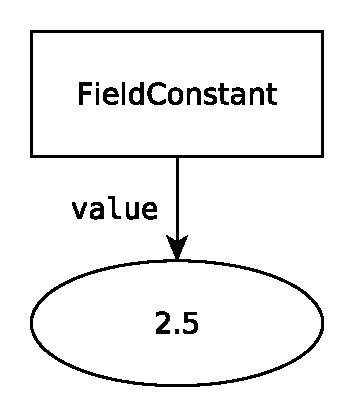
\includegraphics[height=120pt]{../img/autoconversion_array_1_before.pdf}
\end{center}
\end{minipage}
\quad
\begin{minipage}[t]{0.45\linewidth}
\vspace{0pt}
\textbf{Skutečná datová struktura}\\
\vspace{-5pt}
\begin{lstlisting}
value: [2.5]
\end{lstlisting}
\vspace*{-20pt}
\begin{center}
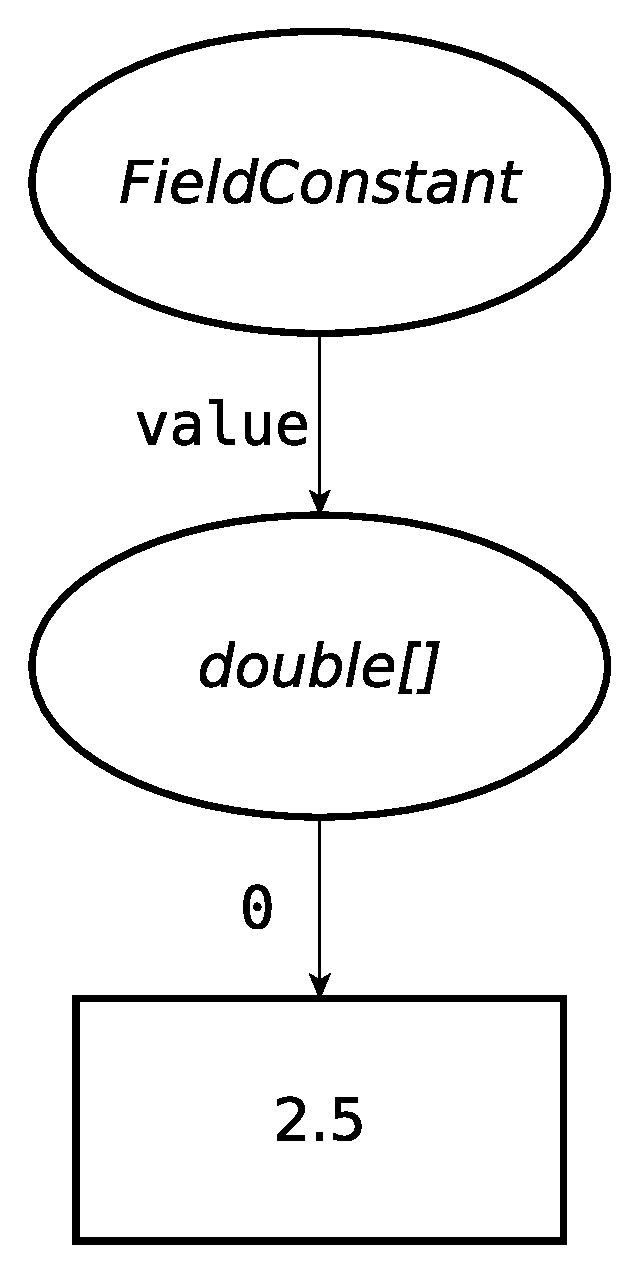
\includegraphics[height=190pt]{../img/autoconversion_array_1_after.pdf}
\end{center}
\end{minipage}
\caption{Autokonverze na jednorozměrné pole}
\label{img:autoconversion_array_1}
\end{figure}	

%TODO desetinna cisla v textu - uvadet s , nebo .?
Obrázek~\ref{img:autoconversion_array_1} znázorňuje autokonverzi hodnoty na jednorozměrné pole. V~klíči \texttt{value} v~záznamu \textit{FieldConstant} se očekává jednorozměrné pole, ale místo něj se na dané pozici vyskytla hodnota \texttt{2.5}. Provede se tedy autokonverze na pole a~poté skutečná datová struktura obsahuje jednorozměrné pole o~jednom prvku, kterým je právě tato hodnota.

Autokonverze na pole funguje obdobně i~pro vícerozměrná pole. Příklad této autokonverze je uveden na obrázku~\ref{img:autoconversion_array_2}. Klíč \texttt{anisotropy} v~záznamu \textit{DarcyFlowMH\_Data} má být dvourozměrné pole. Místo toho se v~datové struktuře vyskytla hodnota. Ta se zkonvertuje na dvourozměrné pole, jehož jediným prvek je právě tato hodnota.

Autokonverze na vícerozměrné pole proběhne i~v~případě, pokud je v~datové struktuře pole o~menší dimenzi, než se očekává. Pokud takový případ nastane, tak se zadané pole zkonvertuje na pole vyšší dimenze obdobně jako to bylo popsáno u~konverzí hodnot na pole.

\begin{figure}[ht]
%\vspace{10pt}
\begin{minipage}[t]{0.45\linewidth}
\vspace{0pt}
\textbf{Zapsaná datová struktura}\\
\vspace{-5pt}
\begin{lstlisting}
anisotropy: 1.5
\end{lstlisting}
\vspace*{-20pt}
\begin{center}
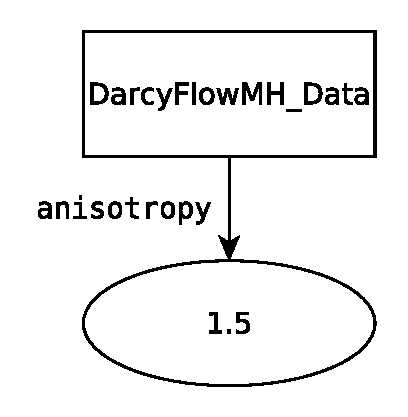
\includegraphics[height=120pt]{../img/autoconversion_array_2_before.pdf}
\end{center}
\end{minipage}
\quad
\begin{minipage}[t]{0.45\linewidth}
\vspace{0pt}
\textbf{Skutečná datová struktura}\\
\vspace{-5pt}
\begin{lstlisting}
anisotropy: [[1.5]]
\end{lstlisting}
\vspace*{-20pt}
\begin{center}
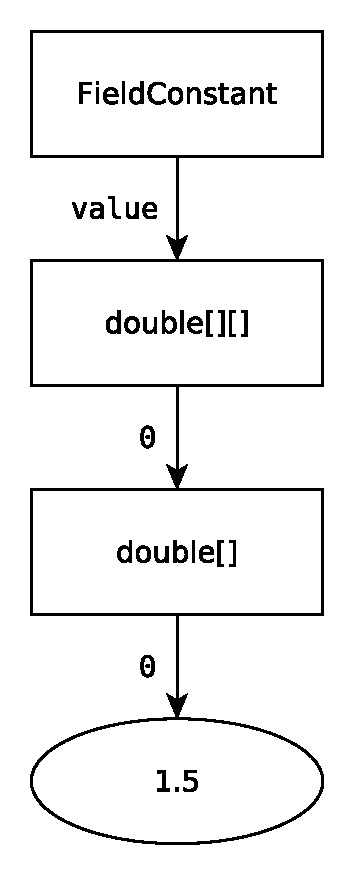
\includegraphics[height=250pt]{../img/autoconversion_array_2_after.pdf}
\end{center}
\end{minipage}
\caption{Autokonverze na vícerozměrné pole}
\label{img:autoconversion_array_2}
\end{figure}	

\subsection{Autokonverze na záznam}
\label{sec:analyza-autokonverze-zaznam}

Autokonverze na záznam se provádí v~případě, že se v~datové struktuře na dané pozici očekává záznam\footnote{Záznam je datový typ, který je odvozený ze základního typu \textit{Record} nebo \textit{Abstract}, viz dále.} a~místo něj se v~datové struktuře nachází pole či primitivní datový typ. Oproti autokonverzi na pole, která proběhne vždy, musí být autokonverze na záznam explicitně povolena ve specifikaci formátu pro daný záznam.

Záznam musí mít ve specifikaci formátu uvedený parametr \texttt{reducible\_to\_key}, který udává, do kterého klíče se má nalezená datová struktura vložit. Pokud tento parametr není uveden, tak záznam autokonverzi nepodporuje a~nelze ji provést.

\begin{figure}[ht]
\begin{minipage}[t]{0.45\linewidth}
\vspace{0pt}
\textbf{Zapsaná datová struktura}\\
\vspace{-5pt}
\begin{lstlisting}
balance: true

\end{lstlisting}
\vspace*{-20pt}
\begin{center}
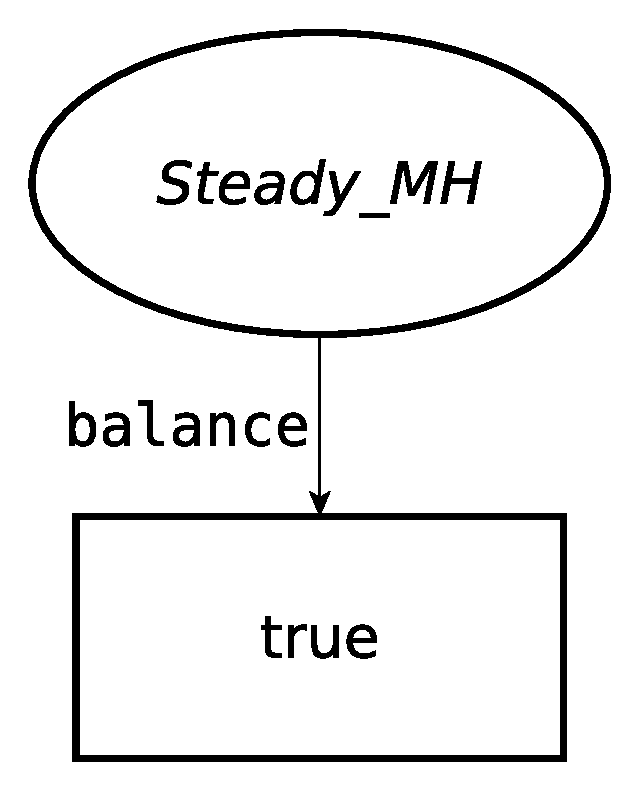
\includegraphics[height=120pt]{../img/autoconversion_record_before.pdf}
\end{center}
\end{minipage}
\quad
\begin{minipage}[t]{0.45\linewidth}
%\centering
\vspace{0pt}
\textbf{Skutečná datová struktura}\\
\vspace{-5pt}
\begin{lstlisting}
balance:
  balance_on: true
\end{lstlisting}
\vspace*{-20pt}
\begin{center}
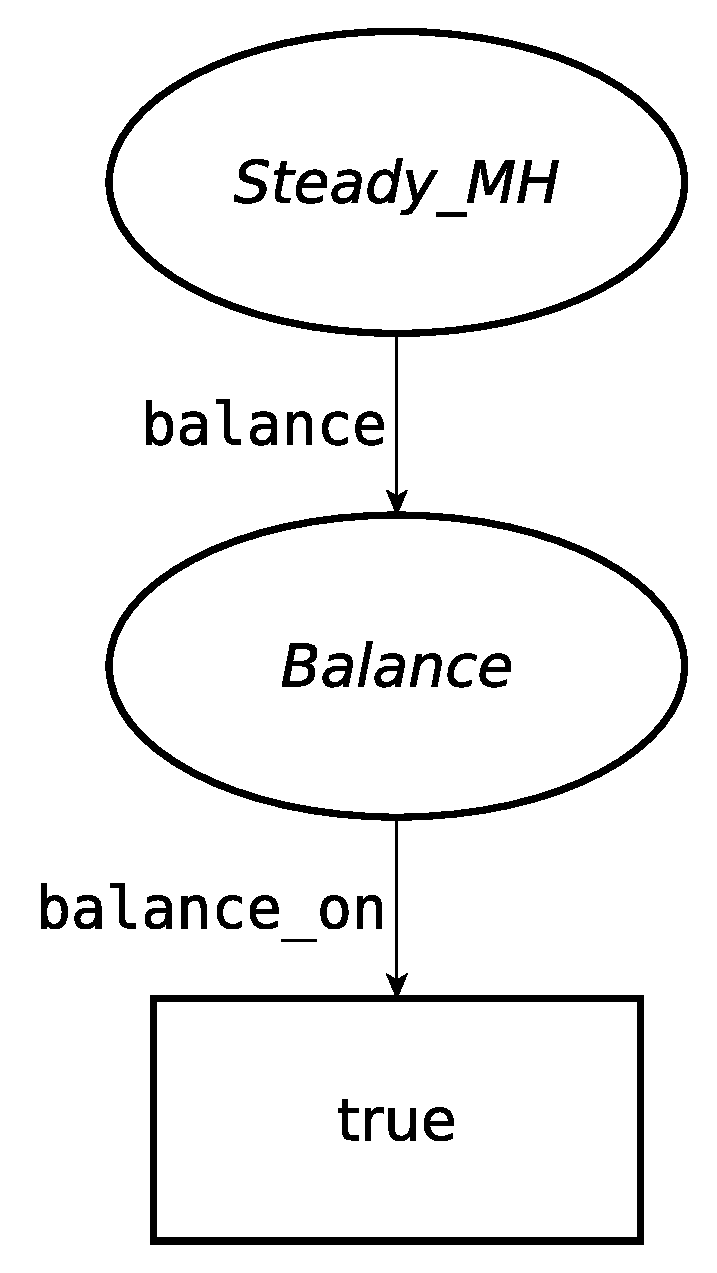
\includegraphics[height=190pt]{../img/autoconversion_record_after.pdf}
\end{center}
\end{minipage}
\caption{Autokonverze na záznam}
\label{img:autoconversion_record}
\end{figure}	

Příklad autokonverze na záznam je znázorněn na obrázku~\ref{img:autoconversion_record}. Záznam \textit{Steady\_MH} obsahuje klíč \texttt{balance}. V~zapsané datové struktuře je pro tento klíč uvedena hodnota \texttt{true}, tedy datový typ \textit{Boolean}. Ovšem podle specifikace formátu se zde očekává záznam typu \textit{Balance}. Jelikož má datový typ \textit{Balance} uveden klíč \texttt{reducible\_to\_key}, který je nastaven na hodnotu \texttt{balance\_on}, tak dojde k~autokonverzi na záznam. Ve skutečné datové struktuře je tedy v~klíči \texttt{balance} záznam typu \textit{Balance}, jehož klíč \texttt{balance\_on} je nastaven na původně uvedenou hodnotu \texttt{true}.

U~záznamů, které podporují tuto autokonverzi, jsou typicky nadefinované výchozí hodnoty klíčů. Uživatel přitom nejčastěji mění právě jeden z~těchto klíčů. Tento klíč je pak ve specifikaci formátu uveden jako \texttt{reducible\_to\_key}. Díky autokonverzi na záznam pak uživatel může měnit hodnotu tohoto klíče bez nutnosti psát název tohoto klíče.

%TODO zalomeni klice?
Existuje speciální případ této autokonverze, kdy se podle specifikace formátu očekává v~datové struktuře abstraktní záznam. Abstraktní záznamy samy o~sobě nepodporují autokonverzi na záznam. Pokud ovšem mají definovaný klíč \texttt{default\_de\-scend\-ant}, který udává výchozí typ záznamu, je možné provést autokonverzi, pokud ji daný záznam podporuje. Tento případ je dále rozebrán v~kapitole \ref{sec:implementace-autokonverze-zaznam}.
%TODO ref

\subsection{Transpozice}
%TODO neni to celkove matouci? je z toho jasne o co se jedna a jak to funguje?
Transpozice je nově přidaná autokonverze, která umožňuje definovat pole záznamů naráz pomocí speciálního zápisu pro jeden záznam. Transpozice může výrazně zkrátit zápis pole záznamů obzvlášť v~případech, kdy záznamy obsahují více klíčů a~mění se pouze hodnoty některých klíčů, zatímco hodnoty ostatních klíčů zůstávají totožné.


\begin{figure}[ht]
\begin{minipage}[t]{0.45\linewidth}
\vspace{0pt}
\textbf{Zapsaná datová struktura}\\
\vspace{-5pt}
\begin{lstlisting}
input_fields:
  region: Region1
  time:
    - 0.5
    - 1.0
\end{lstlisting}
\vspace{-20pt}
\begin{center}
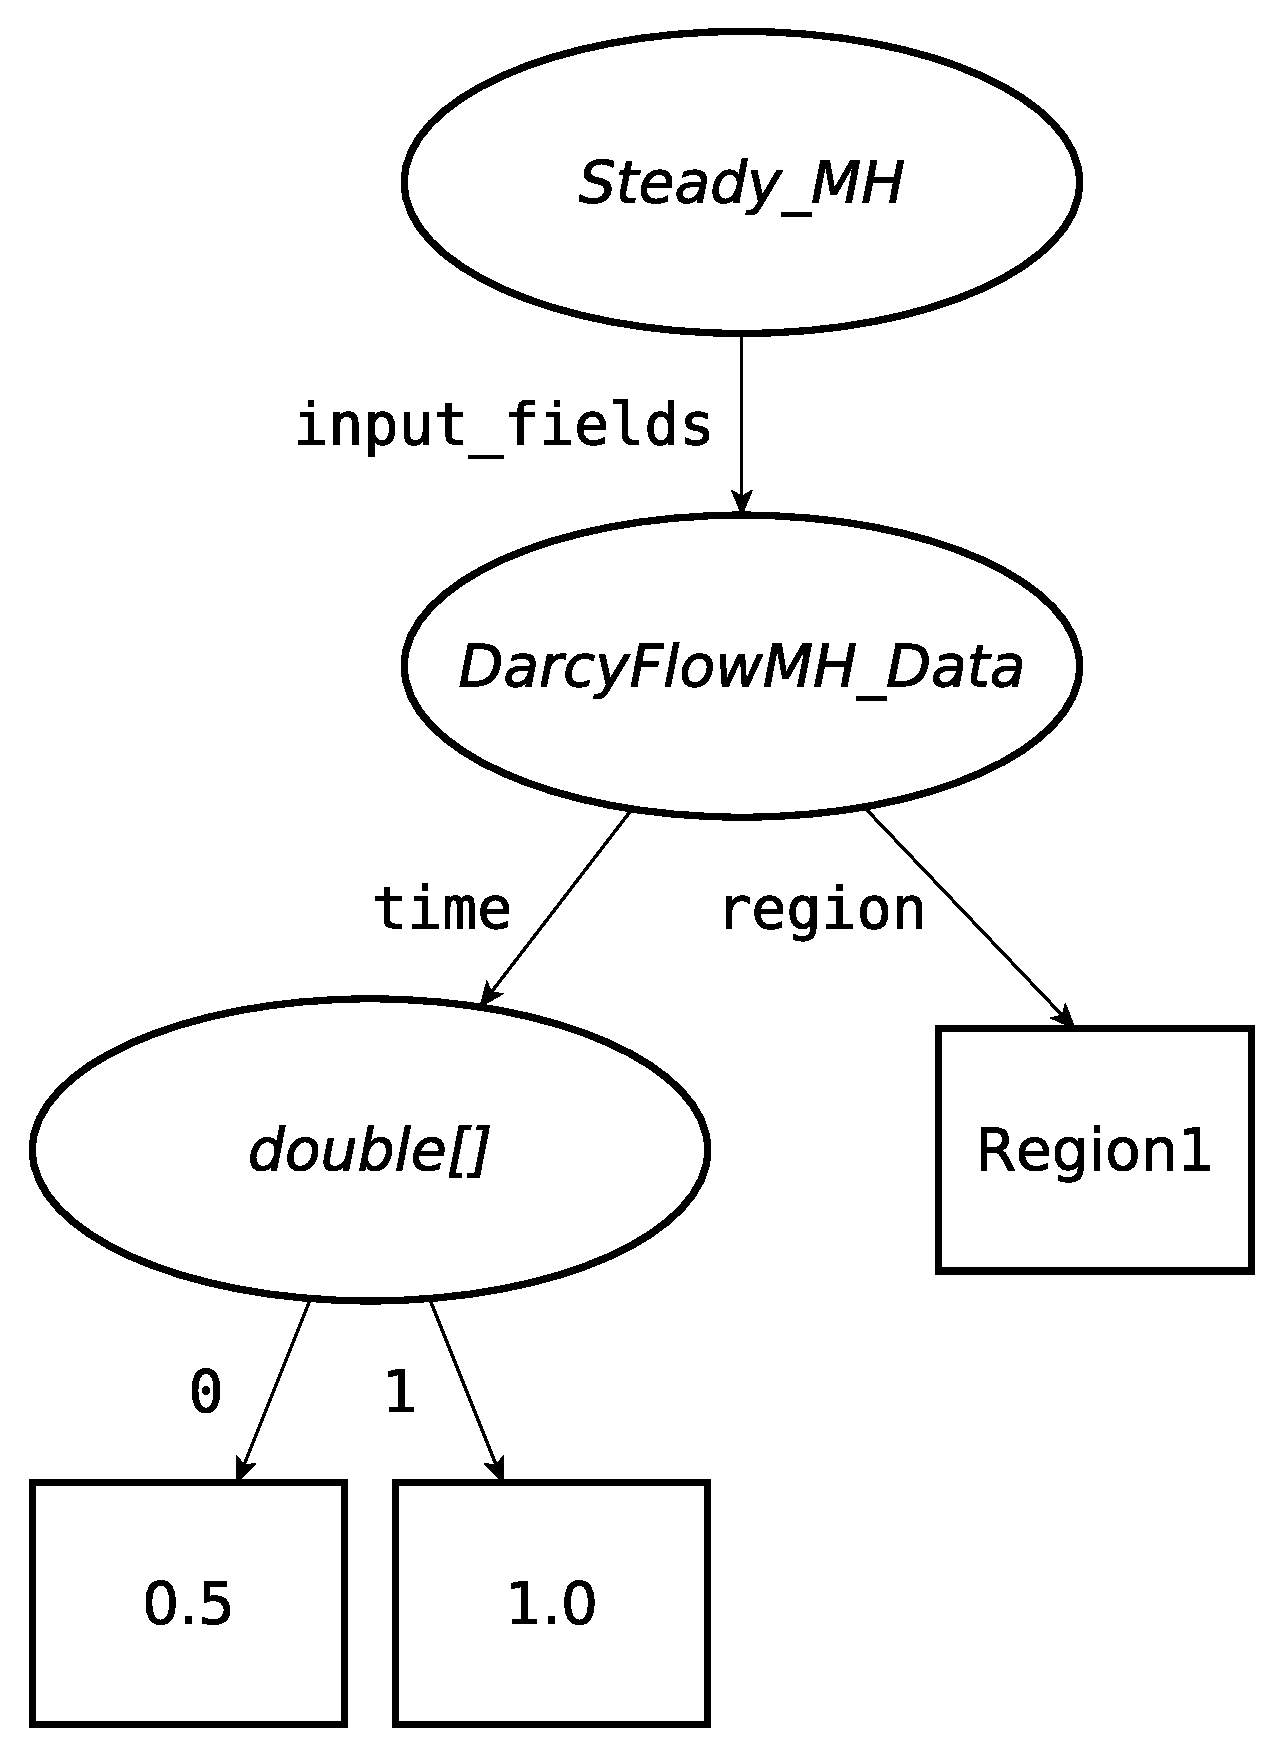
\includegraphics[height=245pt]{../img/autoconversion_transposition_before.pdf}
\end{center}
\end{minipage}
\quad
\begin{minipage}[t]{0.5\linewidth}
\vspace{0pt}
\textbf{Skutečná datová struktura}\\
\vspace{-5pt}
\begin{lstlisting}
input_fields:
  - region: Region1
    time: 0.5
  - region: Region1
    time: 1
\end{lstlisting}
\vspace{-20pt}
\begin{center}
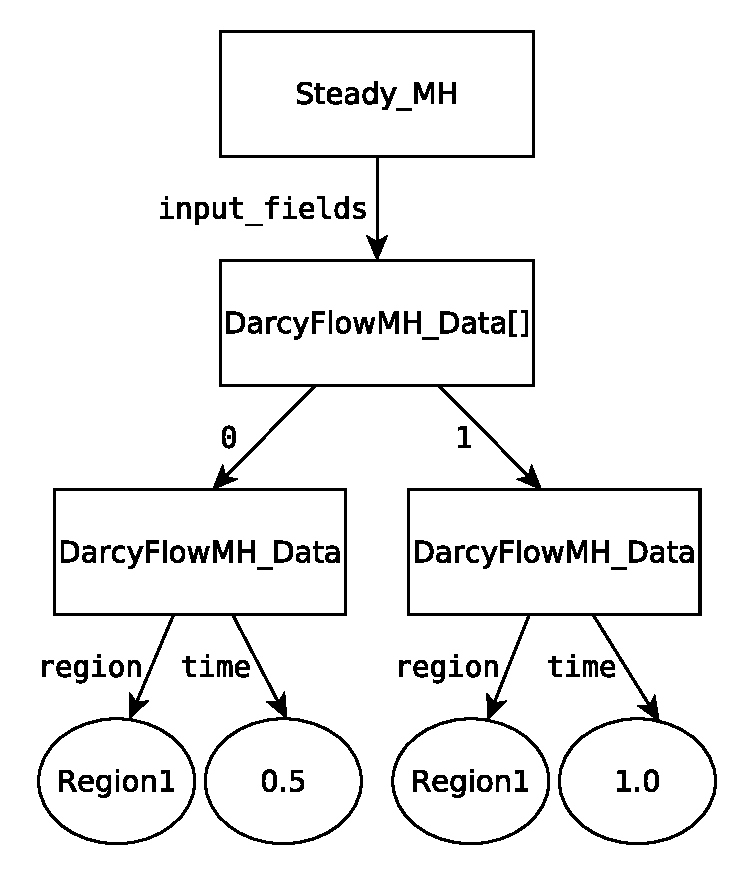
\includegraphics[height=245pt]{../img/autoconversion_transposition_after.pdf}
\end{center}
\end{minipage}
\caption{Autokonverze -- transpozice}
\label{img:autoconversion_transposition}
\end{figure}	

Transpozice je speciálním případem autokonverze na pole. Provádí se v~případě, kdy se v~datové struktuře očekává pole záznamů, ale místo něj je nalezen pouze jeden záznam. Pokud nastane tato situace, proběhnou další kontroly, zda je možné transpozici provést (viz kapitola~\ref{sec:implementace-autokonverze-transpozice}), a~pokud je to možné, tak se zapsaná datová struktura převede následujícím způsobem.

Nejprve se vytvoří pole záznamů, které se očekávalo podle specifikace formátu. Dále se provede expanze polí, kdy se pro každou hodnotu v~poli původně zapsaného záznamu vytvoří samostatný záznam, který se uloží do nově vytvořeného pole záznamů. Během této expanze se do nově vytvořených záznamů vkládají kon\-krétní hodnoty místo původních polí hodnot. Pokud v~daném klíči v~původním záznamu nebylo pole, ale hodnota či jiný záznam, tak se tato hodnota zkopíruje.

%TODO desetinne hodnoty - v obrazku . ale v textu , - jak sjednotit?
Nejjednodušší případ této konverze je znázorněn na obrázku~\ref{img:autoconversion_transposition}. Zde se pomocí transpozice definuje pole \texttt{input\_fields}, které obsahuje záznamy typu \textit{Steady\_MH}. Tento záznam obsahuje klíče \texttt{region} a~\texttt{time}. Zapsaná datová struktura se transponuje tak, že se místo jediného uvedeného záznamu vytvoří pole záznamů o~dvou prvcích, protože pole \texttt{time} obsahuje dvě hodnoty. Každý z~těchto záznamů bude mít klíč \texttt{time} i~\texttt{region}. U~prvního záznamu bude klíč \texttt{time} nastaven na hodnotu~\texttt{0.5}, zatímco u~druhého záznamu bude mít klíč \texttt{time} hodnotu~\texttt{1.0}. Klíč \texttt{region} bude v~obou záznamech nastaven na totožnou hodnotu \texttt{Region1}.
bo
Pokud zapsaný záznam obsahuje více polí, tak jejich expanze probíhá souběžně. První záznam bude tedy obsahovat vždy první prvky z~polí, druhý záznam druhé prvky z~polí atd. To je znázorněno na obrázku~\ref{img:transposition_code_example}. Dále si lze všimnout, že vhodně použitá transpozice může výrazně zkrátit zápis.

\lstset{style=code}

\begin{figure}[ht]
\singlespacing
\begin{minipage}[t]{0.5\linewidth}
\vspace{0pt}
\textbf{Zapsaná datová struktura}\\
\vspace{-5pt}
\begin{lstlisting}
input_fields: 
  region: MyRegion
  bc_type: neumann
  time: [0.5, 1.0, 1.5]
  anisotropy: [2.5, 1.5, 1.8]
\end{lstlisting}
\end{minipage}
\hfill
\begin{minipage}[t]{0.45\linewidth}
\vspace{0pt}
\textbf{Skutečná datová struktura}\\
\vspace{-5pt}
\begin{lstlisting}
input_fields: 
  - region: MyRegion
    bc_type: neumann
    time: 0.5
    anisotropy: 2.5
  - region: MyRegion
    bc_type: neumann
    time: 1.0
    anisotropy: 1.5
  - region: MyRegion
    bc_type: neumann
    time: 1.5
    anisotropy: 1.8
\end{lstlisting}
\vspace*{-20pt}
\end{minipage}
\onehalfspacing
\caption{Ukázka použití transpozice}
\label{img:transposition_code_example}
\end{figure}

\chapter{Návrh}

% big picture - pohled na aplikaci jako celek

\section{Použití syntaxe YAML}

V~kapitole~\ref{sec:analyza-yaml-zapis-datovych-typu} byla uvedena základní syntaxe formátu \gls{YAML}, která se používá pro zápis skalárních hodnot, sekvencí a~map. V~této kapitole je dále upřesněno použití syntaxe \gls{YAML} pro zápis konfiguračních souborů včetně speciálních případů, které se používaly ve formátu \gls{CON}.
%TODO v kapitole X ... v teto kapitole -- o kterou kapitolu se jedna? preformulovat

Formát \gls{CON} měl vyhrazené dva speciální klíče -- \texttt{TYPE} a~\texttt{REF}. První z~nich, klíč \texttt{TYPE}, sloužil pro zadání typu konkrétního záznamu v~datové struktuře abstraktního záznamu. Pomocí klíče \texttt{REF} bylo možné se odkázat na libovolnou část datové struktury.

\subsection{Základní použití syntaxe}

Pro reprezentace primitivních datových typů, polí a~záznamů v~konfiguračních souborech lze jednoduše využít výše popsanou syntaxi formátu \gls{YAML}. Primitivní datové typy lze zapsat s~využitím syntaxe pro skalární hodnoty, pole je možné reprezentovat pomocí syntaxe pro sekvence a~záznamy lze zapsat pomocí syntaxe pro mapy.

Pro reprezentaci polí se doporučuje použít syntaxe pro blokový zápis, kromě případů, kdy je zjednodušený zápis výrazně kratší bez újmy na čitelnosti (např. zápis pole celočíselných hodnot). Pro reprezentaci záznamů se doporučuje používat výhradně syntaxe pro blokový zápis. Zjednodušený zápis záznamů působí chaoticky a~editor nemusí podporovat některé funkce při používání tohoto zápisu.

Formát \gls{YAML} nepředepisuje, jaké by mělo být odsazení při vnořování blokových zápisů, ale pouze vyžaduje, aby bylo v~rámci daného bloku stejné. V~rámci konfiguračních souborů Flow123d se ale doporučuje používat odsazení pomocí dvou mezer, aby byl styl použitý pro zápis konfiguračních souborů jednotný. Editor je optimalizován na použití odsazení pomocí dvou mezer a~znaky tabulátor automaticky převádí na toto odsazení.

\subsection{Abstraktní záznamy}
\label{sec:navrh-yaml-abstrakni-zaznamy}
Abstraktní záznamy jsou datovým typem, který definuje specifikace formátu. Tyto záznamy mohou mít více různých implementací. V~konfiguračním souboru, kde se podle specifikace formátu očekává abstraktní záznam, musí být uvedena konkrétní implementace. Implementace abstraktního záznamu je záznam, který má v~jeho specifikaci uvedeno, že implementuje daný abstraktní záznam. To bylo popsáno v~kapitole~\ref{sec:analyza-specifikace-formatu-abstraktni-zaznamy}.

Příkladem je třeba klíč \texttt{primary\_equation} v~datovém typu \textit{SequentialCoupling}. Typ klíče \texttt{primary\_equation} je \textit{DarcyFlow}, což je abstraktní záznam. V~současné verzi Flow123d existují tři implementace tohoto záznamu -- \textit{Steady\_MH}, \textit{Unsteady\_MH} a~\textit{Unsteady\_LMH}. To znázorňuje obrázek~\ref{img:abstract_record_darcyflow}.

\begin{figure}[h]
	\centering
    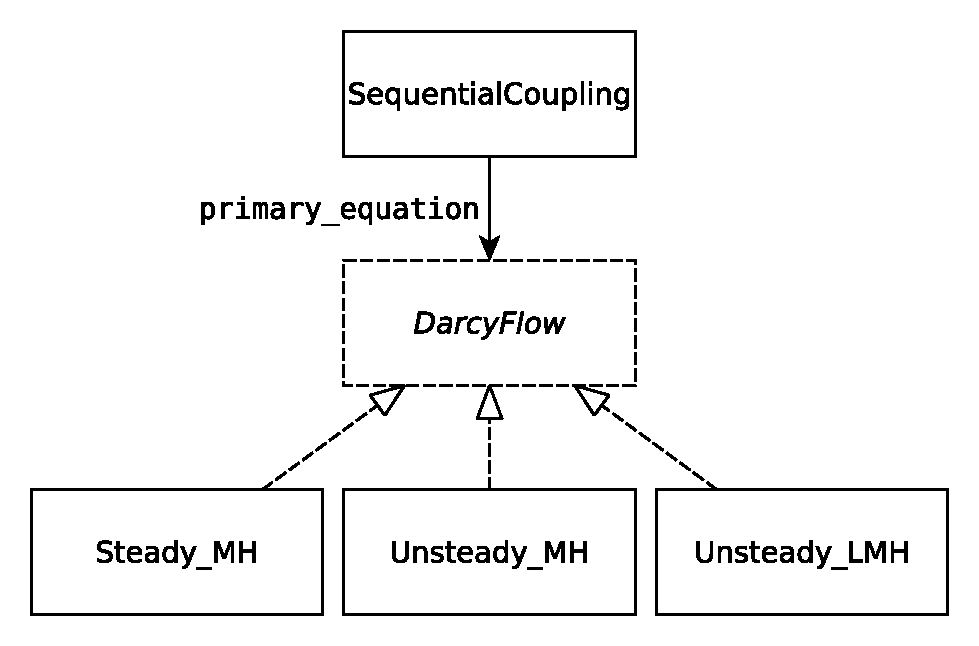
\includegraphics[height=190pt]{../img/abstract_record_darcyflow.pdf}
    \caption{Abstraktní záznam DarcyFlow a~jeho implementace}
	\label{img:abstract_record_darcyflow}
\end{figure}

V~konfiguračním souboru je nutné nějakým způsobem určit, jaká implementace byla zvolena. Formát \gls{CON} toto řešil pomocí speciálního klíče \texttt{TYPE}. Tento klíč obsahoval výběrový typ, který mohl nabývat hodnot, které odpovídaly názvům jednotlivých implementací. Nevýhoda tohoto řešení byla, že klíč \texttt{TYPE} byl uveden v~záznamu jako běžný klíč i~přes to, že pouze určoval datový typ záznamu a~měl jiný význam než ostatní klíče. Ukázka výběru konkrétní implementace ve formátu CON je na obrázku~\ref{img:abstract-record-con} na straně~\pageref{img:abstract-record-con}.

Ve formátu \gls{YAML} existují takzvané tagy, které slouží pro určení datového typu. Jsou definovány některé základní tagy, které se používají pro odlišení typů, které jsou univerzální pro všechny \gls{YAML} dokumenty. Tyto předdefinované tagy byly popsány v~kapitole~\ref{sec:analyza-yaml-zapis-datovych-typu} a~jejich kompletní popis lze nalézt v~dokumentaci formátu YAML~\cite{bib:yaml}. Všechny předdefinované tagy začínají \texttt{!!} (dvěma vykřičníky).

Lze ovšem využít i~uživatelsky definované tagy. Ty začínají pouze jedním znakem~\texttt{!}~(vykřičník) a~poté jsou následovány uživatelsky definovaným názvem. Zpracování těchto tagů je potom aplikačně specifické a~řeší se v~rámci procesu načtení \gls{YAML} dokumentu. Použití uživatelsky definovaného tagu může vypadat následovně.

\lstset{style=short}
\vspace{5pt}
\begin{lstlisting}
solver: !Petsc
  a_tol: 1e-12
  r_tol: 1e-12
\end{lstlisting}
\vspace{-20pt}

Uživatelsky definované tagy jsou ideální pro výběr konkrétní implementace abstraktního záznamu. Jejich zápis je jednoznačně odlišuje od ostatních dat v~záznamu a~nejsou potom součástí samotných dat záznamu. Na obrázcích~\ref{img:abstract-record-con} a~\ref{img:abstract-record-yaml} na straně~\pageref{img:abstract-record-con} lze porovnat způsob výběru implementace abstraktního záznamu ve formátech \gls{CON} a \gls{YAML}.


\subsection{Reference}

Ve formátu CON bylo možné se pomocí referencí odkázat na libovolnou část datové struktury. Tento odkaz byl pak při zpracování nahrazen daty, na které se odkazoval. Dalo se tak předejít duplicitě dat. Pokud některá data byla totožná s daty v jiné části datové struktury, stačilo použít referenci.

Reference se ve formátu CON používala tak, že se do speciálního klíče REF uvedla libovolná cesta do jiné části datové struktury. Ta mohla být buď absolutní nebo relativní a mohla být v libovolné části konfiguračního souboru. Ukázka použití reference ve formátu CON je na obrázku \ref{img:reference-con} na straně \pageref{img:reference-con}.

Formát YAML poskytuje podobnou funkčnost v podobě kotev a aliasů. V libovolné části souboru je možné definovat tzv. kotvu, na kterou je pak možné se odkázat ve zbývající části souboru pomocí aliasu. Kotva začíná znakem \texttt{\&} (ampersand) a za ním následuje její název, který si uživatel může zvolit. Alias začíná znakem \texttt{*} (hvězdička) a za ní je bezprostředně uveden název již existující kotvy. Definice kotvy a použití aliasu může vypadat například následovně.

\vspace{5pt}
\begin{lstlisting}
primary_equation: !Unsteady_LMH
  time: &time
    end_time: 0.5
    max_dt: 0.01
    min_dt: 0.01
time: *time
\end{lstlisting}
\vspace{-20pt}

Použití kotev a aliasů bylo navrženo ve formátu YAML za stejným účelem jako reference ve formátu CON -- ke zrychlení zápisu duplicitních dat.

%TODO zminit operator merge?


\section{Autokonverze}

% vyvojovy diagram - jak se provadi autokonverze - implementace?

\section{Validace}

\section{Kontextová dokumentace}

\section{Automatické doplňování textu}

\section{Funkce editoru}

\section{GUI}


\chapter{Implementace a~testování}


% YAML tab vs spaces - 2 mezery


%TODO zminit odlisnosti ve zpracovani YAML oproti standardnimu chovani - poradi klicu, aliasy, tagy?

% kapitoly obdobne navrhu?
% pouzite knihovny a technologie
% pracovni postupy?
% implementacni uskali
% kdo delal co
% testy

\chapter{Uživatelská příručka}

\section{Zápis konfiguračních souborů pomocí YAML}

\section{Vytváření a~editace konfiguračních souborů}

\section{Validace a~odstranění chyb}

\section{Nastavení} 

%TODO jak odlisit format ve smyslu pouziteho textoveho zapisu vs format semantickeho vyznamu dat (IST) - neco jako XML Schema


%
%
%\section{Konfigurační soubory}
%Priblizeni konfiguracnich souboru a jejich formatu.
%
%Stary format CON a prechod na novy format YAML.
%
%Diskuze XML/YAML(JSON). 
%
%\section{Input Structure Tree}
%Popis formatu datovych souboru.
%
%Definice konkretnich datovych typu.
%
%Specifikovat mozne atributy.
%
%\section{Autokonverze}
%Popsat mozne konverze, uvest do souvislosti s~XML transformacemi?
%
%
%\chapter{Návrh}
%Diagramy pro zpracovani YAML (inspirace SAX vs DOM).
%
%
%
%
%\chapter{Implementace}


\chapter*{Závěr}
\addcontentsline{toc}{chapter}{Závěr}
V~rámci této diplomové práce byl vytvořen editor konfiguračních souborů pro Flow123d. Jedná se o~samostatně funkční aplikaci, která je ovšem navržena s~ohledem na její použití jako součást softwarového balíku GeoMop, který obsahuje další nástroje, které usnadňují práci uživatelům Flow123d.
%TODO zminovat GeoMop?

Editor uživatelům zjednodušuje vytváření a~upravování konfiguračních souborů. Umožňuje ověřit správnost zadané konfigurace pro zvolenou verzi Flow123d a~případně uživatele upozornit na detekované chyby. Tato funkce uživateli přináší časovou úsporu a~uživatelsky příjemnější rozhraní při odhalování chyb.

Editor dále uživatelům poskytuje kontextovou dokumentaci a~našeptávač. Obě tyto funkce přizpůsobují svůj obsah na základě pozice kurzoru v~textu, tedy oblasti, kterou uživatel zrovna upravuje. Pro uživatele to představuje značné zjednodušení, jelikož může využít tyto funkce místo prohledávání rozsáhlé dokumentace.

V~neposlední řadě editor obsahuje komponentu pro grafické znázornění datové struktury, která poskytuje alternativní pohled na zadaná data, a~umožňuje rychlejší orientaci v~rozsáhlých konfiguračních souborech. Kromě těchto stěžejních funkcí editor poskytuje i~běžné nástroje pro manipulaci s~textem, jako jsou například operace se schránkou, možnost vracení provedených změn, vyhledávání a~nahrazení nebo změna úrovně odsazení.

%TODO zmenit formulaci
%TODO zminit GPL + odkaz na zdrojove kody
Aplikace je multiplatformní a~podporuje systémy Windows (XP nebo novější) a~Linux. S~ohledem na požadavek multiplatformní aplikace byl pro vývoj použit jazyk Python~3 a~grafická knihovna PyQt~5. K~aplikaci byly vytvořeny instalační balíčky pro Windows a~Debian.

V~rámci budoucího vývoje jsou plánovány další dodatečné funkce. Jedná se např. o~zlepšení zvýraznění syntaxe, které se by se mohlo přizpůsobit přímo formátu Flow123d. Další možné vylepšení spočívá v~rozšíření funkcionality komponenty pro vizualizaci datové struktury. Ta by mohla v~budoucnu podporovat kromě zobrazení i~editaci dat nebo vylepšené zobrazení speciálních datových typů.

\begin{thebibliography}{9}
% set url to non-mono style
\urlstyle{same}

\addcontentsline{toc}{chapter}{\bibname}

\bibitem{bib:ecma404}
\textit{Standard ECMA-404: The JSON Data Interchange Format}. [online]. Geneva: Ecma International, 2013. [cit. 2016-02-23] Dostupné z: \url{http://www.ecma-international.org/publications/files/ECMA-ST/ECMA-404.pdf}

\bibitem{bib:flow123d-manual}
BŘEZINA, Jan et al. \textit{Flow123d version 1.8.2: Documentation of file formats and brief user manual}. [online]. Liberec, 2015 [cit. 2016-02-24]. Dostupné z: \url{http://flow.nti.tul.cz/packages/1.8.2_release/flow123d_1.8.2_doc.pdf}

\bibitem{bib:sgml-iso}
\textit{ISO 8879}. Amd.1:1988. International Organization for Standardization, 1988. [cit. 2016-02-26]. 

\bibitem{bib:xml}
\textit{Extensible Markup Language (XML) 1.0}. Fifth Edition. [online]. W3C, 2008. [cit. 2016-02-26]. Dostupné z: \url{http://www.w3.org/TR/2008/REC-xml-20081126}

\bibitem{bib:yaml}
BEN-KIKI, Oren et al. \textit{YAML Ain’t Markup Language (YAML™) Version 1.2}. 3rd Edition. [online]. 2009. [cit. 2016-03-06]. Dostupné z: \url{http://www.yaml.org/spec/1.2/spec.html}


\end{thebibliography}

\appendix
\counterwithin{figure}{chapter}

\chapter{Ukázky kódů konfiguračních souborů}

\lstset{style=code}

\begin{figure}[h]
\begin{lstlisting}
{
  solver = {
    TYPE = "Petsc",
    a_tol = 1e-12,
    r_tol = 1e-12
  }
}
\end{lstlisting}
\vspace*{-20pt}
\caption{Výběr implementace abstraktního záznamu ve formátu CON}
\label{img:abstract-record-con}
\end{figure}

\begin{figure}[h]
\begin{lstlisting}
solver: !petsc
  a_tol: 1e-12
  r_tol: 1e-12
\end{lstlisting}
\vspace*{-20pt}
\caption{Výběr implementace abstraktního záznamu ve formátu YAML}
\label{img:abstract-record-yaml}
\end{figure}

\clearpage

\begin{figure}[h]
\begin{lstlisting}
{
  primary_equation = {
    TYPE = "Unsteady_LMH",
    ...
    time = {
      end_time = 0.5, 
      max_dt = 0.01,
      min_dt = 0.01
    }
  },
  
  time = {
    REF = "../primary_equation/time"
  }
}
\end{lstlisting}
\vspace*{-20pt}
\caption{Použití reference ve formátu CON}
\label{img:reference-con}
\end{figure}

\begin{figure}[h]
\begin{lstlisting}
primary_equation: !Unsteady_LMH
  ...
  time: &time
    end_time: 0.5
    max_dt: 0.01
    min_dt: 0.01

time: *time
\end{lstlisting}
\vspace*{-20pt}
\caption{Použití reference ve formátu YAML}
\label{img:reference-yaml}
\end{figure}


\end{document}
